\chapter{Work Done}


\section{Introduction}
This chapter discusses the implementation i.e the algorithm used to design this system and and the result. It also dicusses the analaysis of designed system and the screenhots of the implemented system. 



\section{Implementation}
\subsection{Algorithm}
\vspace*{2 ex}
The implemented algorithm takes eight words as input and results in 10x10 matrix crossword puzzle and hints for game as output. Two variables to keep track of last horizontal and vertical indexes occupied by the character are maintained and an integer list (predefined datastructure) to store the indexes of column that are verically occupied by other words whose character matches with the characters placed in first row.
\vspace*{2 ex}

The steps involved in the algorithm are as follows : 
\vspace*{2 ex}
\begin{enumerate}
\setlength{\itemsep}{-0.3em}
\item Arrange the random words selected in descending order of words length.
\item Longest word is placed in the first row horizintally and a variable is maintained to keep track of the horizontal index next to the last character. 
\item \quad Check if next word can fit in first row.
\item \quad\quad If it can be placed in first row then it will be placed their.
\item \quad\quad Else check if the first character of next word to be placed matches any character of word(words) already placed in first row.
\item \quad\quad\quad If it matches then word is placed vertically and a variable is maintained to keep track of vertical index next to last character.
\item \quad\quad\quad Else word is stored in String array say, "x"
\item Half of the words in array "x" are placed vertically from the last index occupied by characters in first row
\item Rest half are placed horizintally from the last index occupied by any character vertically starting from any random horizontal index
\end{enumerate} 

\vspace*{6 ex}
Here is the sample output of implemented algorithm :

\begin{figure}[!ht]
\centering
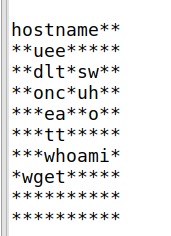
\includegraphics[scale=0.6]{algo.png}
\caption{\label{img5} Puzzle Interface }
\end{figure}



\section{Result}
A crossword puzzle generation system has been designed that can generate many random crossword puzzles.

\vspace*{2 ex}
\section{Analysis}
\textbf{LIMITATIONS :}


On analysis, it has been found that the implemented crossword puzzle system has the following limitations :\vspace*{2 ex}
\begin{enumerate}
\item If first chatacter of words doesn't matches any chatacter placed in first row then puzzle will not be an effecient.
\item Algorithm doesn't matches any characters except for the first one to generate puzzle.
\item Crossword puzzle can only be generated for words less than or equal to 10.
\item Number of words generated in puzzle depends on the length of word. If words with longer length(more than 5) are more, less number of words will be generated  in puzzle. 
\end{enumerate}


\section{How to use}
In order to use this crossword puzzle generation system; Eclipse, pgsql and pqsql connector are required.


\section{Screenshots}
\subsection{Welcome Page}
This is the welcome page to greet users and ask them to start the crossword puzzle. 
\begin{figure}[!ht]
\centering
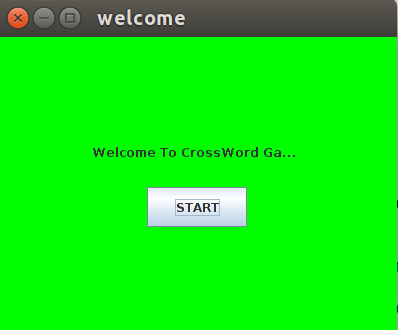
\includegraphics[scale=0.6]{first.png}
\caption{\label{img5} Welcome Page}
\end{figure}
\newpage


\subsection{Generated Puzzle}
This the second window where user will be directed after clicking the "start" button of first window. On clicking the "Generate Game", the puzzle and the hints will be generated.  
\begin{figure}[!ht]
\centering
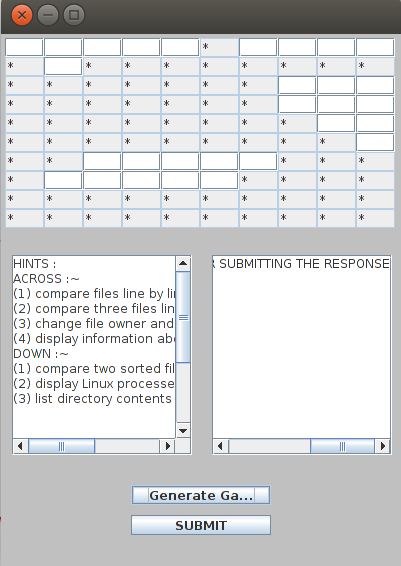
\includegraphics[scale=0.6]{puzzle.png}
\caption{\label{img5} Generated Puzzle with hints}
\end{figure}
\newpage

\subsection{Generated Puzzle with solution}
Answer for the puzzle will be generated on submitting the guessed answer by user in second window itself as shown below. 
\begin{figure}[!ht]
\centering
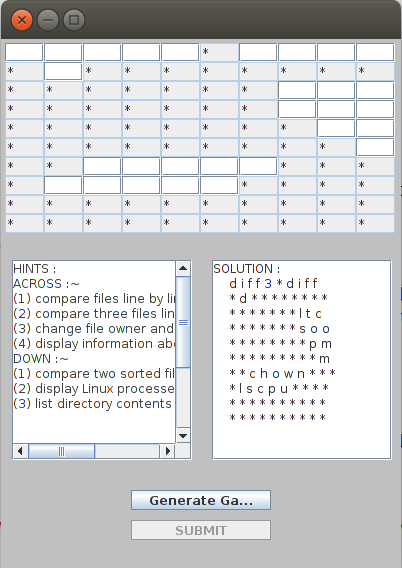
\includegraphics[scale=0.6]{sol.png}
\caption{\label{img5} Puzzle with solution }
\end{figure}




